\documentclass[Main.tex]{subfiles}

\begin{document}
\section{Methodology for Designing a Swarm Robot Control Algorithm}

This section describes a particular methodology for designing and modeling robot controllers that is widely used in the swarm robotics community. While this is by no means the only modeling method available for robot swarms---e.g., other (related) modeling and control methods are described in \cite{Bayazit2005, Berman2007, Billard1999, Sugawara2013}---it has the important property of being an iterative method that integrates multiple levels of abstraction of the multi-agent system. This opens up the opportunity for parameter discovery  and optimization, which I am particularly interested in and is covered in section~\ref{sec:opt}.

Some early work related to modeling swarm robot systems was done by Martinoli et al.\cite{Martinoli1995, Martinoli2004} outlining collective group behaviors and the associated system dynamics by studying two distinct swarming tasks. The first task involved the aggregation of sticks by teams of robots in a closed environment while the second experiment was a team-based, collaboration task where groups of two robots were used to pull long sticks out of the ground. The second experiment has been widely studied and extended upon by numerous researchers like Martinoli, Mondada, Ijspeert, Lerman, and Correll in the past decade and is well known in the community as the ``Stick Pulling Experiment''. We will use this experiment as a recurring example throughout this section to introduce new concepts, beginning with a general procedure for designing the robot controller. If the reader is not familiar with the stick pulling experiment, a brief description is available in section~\ref{sec:stickpull} and is recommended before continuing with this section.

\subsection{Experiment Setup}
The first step in the robot controller design methodology is to describe the swarming task being studied. The general strategy used by each individual agent in the swarm is defined and later translated into a viable microscopic model. A hypothesis for the observed, collective behavior of the swarm is also supplied, which is later quantified into a mathematical macroscopic model.

Physical characteristics of the swarm system are generally described in the experiment setup as well. These may include environmental variables such as arena size, agents properties such as speed, communication and sensing radii, the computation power of each individual in the swarm, etc. This is an important step in identifying the important system parameters that affect the outcome of the experiment, versus the environmental and agent based values that can be abstracted away when designing micro and macro-level models.
 

\subsection{Designing the Controller Construct}
With this experiment setup in mind we will now discuss designing the robot controller. The first step in this process is to create a logic construct---a flowchart, state-machine or algorithm that describes the desired robot behavior for the given task.

The original robot controller for the stick pulling experiment was designed as a flowchart seen in Figure~\ref{fig:stickchart}. The rectangular boxes in the flowchart are states that the robot controller can be in while the rhomboid shapes signify decision processes within the controller. The result of each decision process is dependent on several factors, for example, the \emph{object detected?} decision depends on feedback from the robot's IR proximity sensors. The \emph{obstacle?} decision depends on the output produced by the sensory neural net of the agent (see Figure~\ref{fig:khepschem}). The \emph{obstacle?} decision happens when the robot has an object in front of it and must decide whether it is an obstacle such as another robot or wall, or a target such as a stick. As one can imagine, the output from the neural net is not always correct due to factors like the distance and angle of incidence between the detecting robot and the object in front of it, as well as sensor noise.

\begin{figure}[!tp]
\centering\includegraphics[width=10cm]{stickControl.png}
\centering\caption{Flowchart for an individual robot controller in the stick pulling experiment.}\label{fig:stickchart}
\end{figure}

\begin{figure}[!tp]
\centering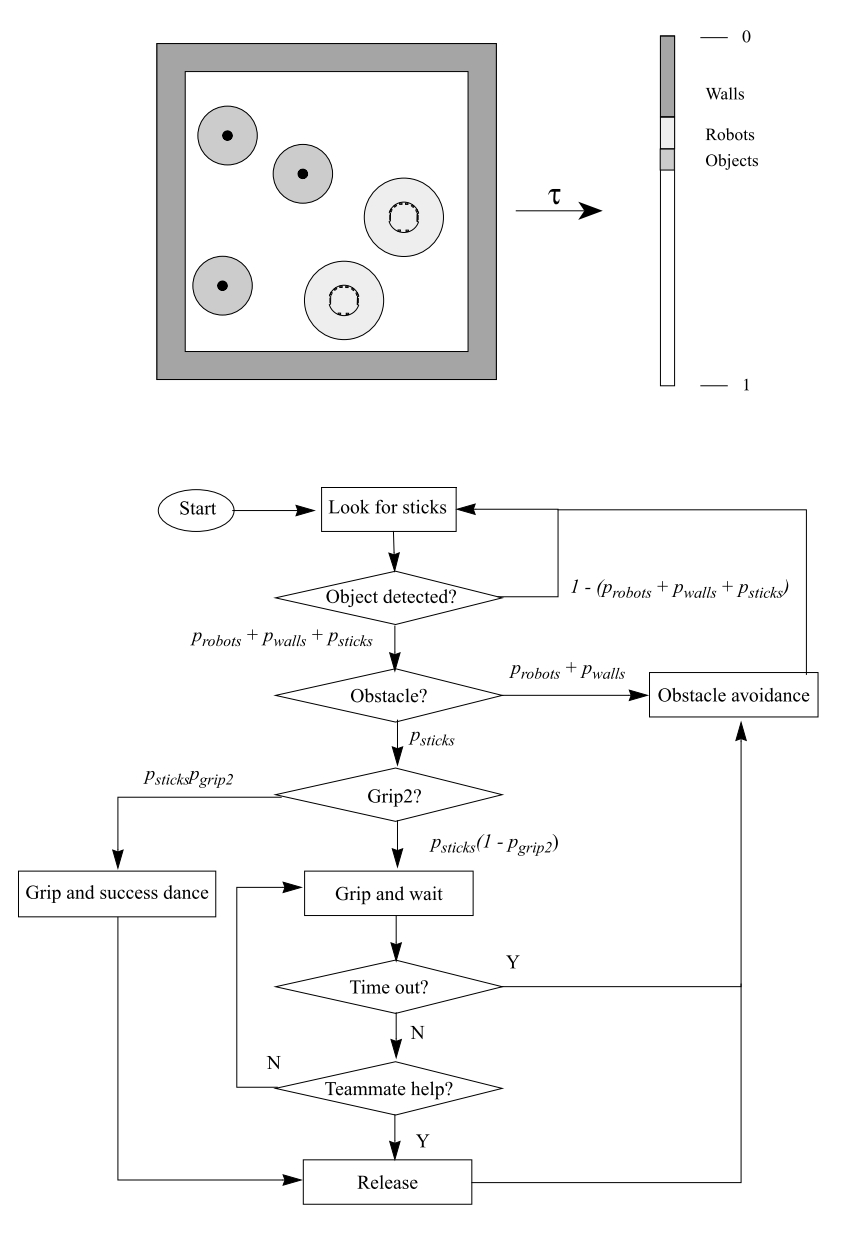
\includegraphics[width=12.5cm]{stickprobcontrol.png}
\centering\caption{\textbf{Top:} A visualization of the conversion function $\boldsymbol{\tau}:\mathbb{R}^2_{\geq0} \rightarrow \mathbb{R}_{\geq0}$, going from a 2D physical space to a 1D probability space. \textbf{Bottom:} Flowchart of a robot controller in the probabilistic model of the stick pulling experiment. $p_{robots} =$ probability of encountering teammates; $p_{walls} =$ probability of encountering walls; $p_{sticks} =$ probability of encountering one of the sticks; $p_{grip2} =$ probability to make a grip2} \label{fig:probstickchart}
\end{figure}

Given this stochastic nature of decision processes in the flowchart, it makes sense for us to assign them probabilities of traversal. We therefore convert a physical 2D arena space into a 1D probability space via a transformation function, $\boldsymbol{\tau}:\mathbb{R}^2_{\geq0} \rightarrow \mathbb{R}_{\geq0}$, (top of Figure~\ref{fig:probstickchart}). The probabilities, $p_{robots}$, $p_{walls}$, etc., seen in the flowchart are computed using simple geometric properties of the environment. For example, $p_{walls}$ is computed as the ratio between the area where a robot can sense the wall (the dark gray perimeter of the square seen in top Figure~\ref{fig:probstickchart}) and the area of the whole arena.

You may notice that in Figure~\ref{fig:probstickchart} there are still some deterministic decision processes, such as \emph{time out?}. The \emph{time out?} decision process is special as it deals with an internal state variable in the agent, namely, its timer value. Such deterministic decision processes make the mathematical system more complex because of the need to maintain the current state of each agent instead of the collective state of the whole system. As we will discuss later, there are ways to stochastically model these deterministic decision processes (thereby simplifying the mathematical model) without loss of generality and without affecting the solution of the system in equilibrium, if one exists. 

The use of a flowchart makes it straightforward to describe the robot controller but doesn't do a very good job of exposing the true stochastic nature of the system, nor does it allude to the possibility of a mathematical model for the system. And so, we exchange this simple construct for a more mathematically robust one---a finite state machine (FSM).

When studying non-spatial models, the robot controller can be characterized by an FSM with a discrete number of states under urgent, time-step driven semantics, as seen in Figure~\ref{fig:allfsm}. Just like the flowchart, the states in the FSM ($A, B, C$ \& $D$) represent physical states that the robot can be in, such as  \emph{searching}, \emph{waiting}, etc. One can think of each state as being an \emph{action} that the robot is currently performing based on stimulus from the environment and other robots. These stimuli can cause a robot to transition from one state to another and are represented as \emph{conditionals} on the edges of the FSM, $c_i$. These conditionals are equivalent to the decision process blocks in the flowchart and can be derived from:
\begin{enumerate}
\item Sensor readings (or stigmergy) and explicit communication, e.g., seeing red light through an rgb sensor or seeing a certain number of robots around you,
\item internal timers, e.g., transition back to search after waiting for 3 seconds,
\item or a combination of both, e.g., transition back to search after waiting for 3 seconds \emph{iff} you see no other robots in your vicinity, otherwise, reset your timer.
\end{enumerate}

We can now extend this modeling framework of robot behavior as an FSM to construct a Probabilistic Finite State Machine (PFSM), where the conditionals in the FSM are no longer \emph{true/false} values but instead are probabilities of transitioning from one state to another based on external stimulus or internal state. 

As alluded to earlier, the case of a state transition based on an internal timer is especially interesting. Let $c_1$ in Figure~\ref{fig:fsm} be the condition $t_A \geq 5$, i.e. time in state $A$ is greater than or equal to 5 time steps (or ticks). This conditional is true when the robot has remained in state $A$ for at least 5 ticks and consequently transitions to state $B$. Thus, the conditional $c_1$ says a robot may remain in state A for no more than 5 ticks. The equivalent transition probability for this condition would be $p_1 = 1/5$. Therefore, at each time step of the PFSM simulation, there is a $1/5$ chance that the robot will transition from state A to state B. The expected number of ticks before a transition happens is then equal to 5. This transition from deterministic FSM models to probabilistic PFSM models for swarm robot algorithms is discussed in further detail in\cite{Correll2008}.
 
\begin{figure}[!t]
\centering
	\begin{subfigure}[t]{.4\textwidth}
		\centering\begin{tikzpicture}[->,>=triangle 45,shorten >=2pt,auto,node distance=3cm,
 	                   semithick]

 		\node[state] (1) {$A$};
 	 	\node[state] (2) [right of=1] {$B$};
 		\node[state] (3) [below of=2] {$C$};
	  	\node[state] (4) [below of=1] {$D$};

		\begin{scope}
		  \path (1) 	edge node[below]{$c_1$} (2)
  			          	edge node{$c_2$} (3)
				 (2)	edge node{$c_3$} (3)
						edge[bend right] node[above]{$c_4$} (1)
				 (3) 	edge node{$c_5$} (4)	
				 (4) 	edge node{$c_6$} (1);
		\end{scope}
		\end{tikzpicture}
	\caption{FSM representing a single robot controller with conditional edge transitions that depend on internal and environmental factors such as timers, sensor readings, etc. Vertices represent physical or internal states that a robot can be in.}\label{fig:fsm}
	\end{subfigure}~
	\begin{subfigure}[t]{.4\textwidth}
		\centering\begin{tikzpicture}[->,>=triangle 45,shorten >=2pt,auto,node distance=3cm,
                    semithick]

 		 \node[state] (1)              {$A$};
 		 \node[state] (2) [right of=1] {$B$};
		 \node[state] (3) [below of=2] {$C$};
		 \node[state] (4) [below of=1] {$D$};

		\begin{scope}
		  \path (1) 	edge node[below]{$p_1$} (2)
  			          	edge node{$p_2$} (3)
				 (2)	edge node{$p_3$} (3)
						edge[bend right] node[above]{$p_4$} (1)
				 (3) 	edge node{$p_5$} (4)
				 (4) 	edge node{$p_6$} (1);
		\end{scope}
	\end{tikzpicture}
	\caption{PFSM of a robot controller with probabilistic edge transitions derived from simple geometric properties of the system.}\label{fig:pfsm}
	\end{subfigure}
	\begin{subfigure}[t]{.4\textwidth}
		\centering\begin{tikzpicture}[->,>=triangle 45,shorten >=2pt,auto,node distance=3cm,
                    semithick]

 		 \node[state] (1)              {$N_A(t)$};
 		 \node[state] (2) [right of=1] {$N_B(t)$};
		 \node[state] (3) [below of=2] {$N_C(t)$};
		 \node[state] (4) [below of=1] {$N_D(t)$};

		\begin{scope}
		  \path (1) 	edge node[below]{$p_1$} (2)
  			          	edge node{$p_2$} (3)
				 (2)	edge node{$p_3$} (3)
						edge[bend right] node[above]{$p_4$} (1)
				 (3) 	edge node{$p_5$} (4)
				 (4) 	edge node{$p_6$} (1);
		\end{scope}
	\end{tikzpicture}
	\caption{A macroscopic model for the swarm system as a whole. Vertices, $N_{s_i}(t)$, represent the number of robots in state $s_i$ at time $t$. Edges are still transition probabilities between states but can also be thought of as proportions of agents entering or leaving a state at time $t$.}\label{fig:pfsmmacro}
	\end{subfigure}
\caption{Transitioning from, \textbf{(a)}: micro-model FSM that describes a single robot controller, to \textbf{(c)}: macro-model PFSM that characterizes the entire swarm system.}\label{fig:allfsm}
\end{figure}

\subsection{Mathematical Description of the System}
Given a discrete set of states and conditions for transitions between them, usually in the form of probabilities of transition, a \emph{master equation} defines a set of ordinary differential equations that describe the time evolution of a physical system. So far, we have used logical constructs like the FSMs to represent the robot controller running within each individual agent of the swarm system. We could instead look as these constructs as a model for the entire system, in which case the vertices of the FSM become accumulators of robots currently in a state and the edges define fractions of agents entering or leaving a given state at time $t$. The PFSM now becomes a macroscopic definition of the robot swarm and can be used to define a mathematical model for the time evolution of the system.

We will shortly discuss the conditions for linearity in a swarm system but for now, assume a simple master equation of the form,
\begin{equation}
\D{\vec{P}(t)} = \mathbf{A}\vec{P}(t)\label{eq:firstmaster}
\end{equation}
$\vec{P}$ is a vector containing $p_i(t)$, $i = [1, \ldots, |P|]$, the time-dependent probability of being in state-$i$ in the corresponding PFSM. $\mathbf{A}$ is a matrix containing transition rates of going from state-$i$ to state-$j$ in the PFSM. When we multiply both sides of equation~\eqref{eq:firstmaster} by the total number of agents, $N_0$, we get the modified master equation that gives a macroscopic description of the system.
\begin{align}
N_0 \vec{P}'(t) = \mathbf{A}\left(N_0\vec{P}(t)\right)\notag\\
\vec{S}'(t) = \mathbf{A}\vec{S}(t)\label{eq:master}
\end{align}
where $\vec{S}$ is a state vector containing the number of agents in each state, $N_{s_i}$, at time t. Here, $\abs{\vec{S}}$ is equal to the number of unique states of the system, e.g. $\abs{\vec{S}} = 4$ in our previous PFSM example from Figure~\ref{fig:pfsm}. The matrix $\mathbf{A}$ contains transition probabilities between the states in the PFSM. There a two types of elements, $a_{ij}$ in matrix $\mathbf{A}$.
\begin{enumerate}
\item The non-diagonal entries, $a_{ij}$ s.t. $i\not=j$, are equal to $p(c_{ij})$ (shortened to $p_{ij}$), the probability of transitioning from state $s_i$ to $s_j$ via the edge with conditional $c_{ij}$ in the FSM.
\item The diagonal entries, $a_{ii}$, are equal to the negative sum of all edge probabilities $p_{ij}$ leaving state $s_i$.
\end{enumerate} 
If an edge does not exist between two states $s_i$, $s_j$ ($i\not=j$) in the FSM, then entry $a_{ij} = 0$, e.g., the master equation for the swarm system described in Figure~\ref{fig:pfsm} is,
\begin{equation}\label{eq:mastereqns}
\left(
	\begin{array}{c}N_A'(t) \\ N_B'(t) \\ N_C'(t) \\ N_D'(t)\end{array}
\right) =
\left(
	\begin{array}{cccc}
	-(p_1 + p_2) & p_4 & 0 & p_6\\
	p_1 & -(p_3 + p_4) & 0 & 0\\
	p_2 & p_3 & -p_5 & 0\\
	0 & 0 & p_5 & -p_6
	\end{array}
\right)
\left(\begin{array}{c}N_A(t) \\ N_B(t) \\ N_C(t) \\ N_D(t)\end{array}\right)
\end{equation}

In most of the scenarios being discussed in this paper, we assume that agents are neither removed nor added to a swarm system once an experiment has begun and therefore add the following constraints to the model,
\begin{align}
N_0 = & \sum\limits^{\abs{\vec{S}}}_{i=1} N_i(t)\\
\forall i \gets 1\ldots\abs{\vec{S}}, & \sum\limits^{\abs{\vec{S}}}_{j=1}a_{ij} = 1 \hspace{1cm}\text{(in matrix $\mathbf{A}$)}
\end{align}
Due to this constraint a simplification can be made to any one (but no more than one) of the states $s_i$ in $\vec{S}$ so that,
\begin{equation}
	N_{s_i}(t) = N_0 - \sum\limits^{j=1,j\not=i}_{\abs{\vec{S}}}N_{s_j}(t)
\end{equation}

In swarm robotics literature, the master equation is often expanded to a set of difference equations (DEs) or continuous ODEs called \emph{rate equations} of the form,
\begin{equation}\label{eq:rateeqns}
	N_{s_i}'(t) = \sum\limits_{j=1}^{\abs{\vec{S}}}p_{ji}N_{s_j}(t) - \sum\limits_{k=1}^{\abs{\vec{S}}}p_{ik}N_{s_i}(t)
\end{equation}
along with a set of initial conditions that define the number of robots in each state, $s_i$, at time $t = 0$. Rate equations are the preferred method for describing a macro-model of a swarm system because, unlike the master equation, they can represent probability values that could be complex, non-linear functions of environment variables, control variables, as well as time. These are also referred to as population dynamics models, or PDMs.

\subsection{Microscopic Simulation of the System}
One of the advantages of using macroscopic, mathematical models for describing robot swarms is their ability to predict the state of the system at equilibrium, if it exists. But given the phenomenological approach to designing macro-models, it may not always be intuitive to construct the math equations to accurately describe the system. This is especially true in the case of spatial macro-models, which we will discuss later. Even if the rate equations are defined, the system may not be easily solvable, either analytically or numerically. Fortunately there is another modeling tool that comes to our aid in such situations. 

The Microscopic model (or micro-model) of a swarm system can be simulated using the \emph{Gillespie} simulation technique\cite{Gillespie1976, Gillespie1977}. Here, each agent is simulated individually using dice rolls and probability. Gillespie developed this simulation algorithm in the 1970s to model the time evolution of reactant and product volumes in a chemical reaction. The individual agents in his chemical system were single molecules of the reactant and the micro-model was derived from the dynamics of molecule interactions. The probability of two reactant molecules colliding was computed using simple physical properties such as the radius and velocity of the molecules in the reaction medium\cite{Gillespie1976}. 
\begin{figure}[!t]
\centering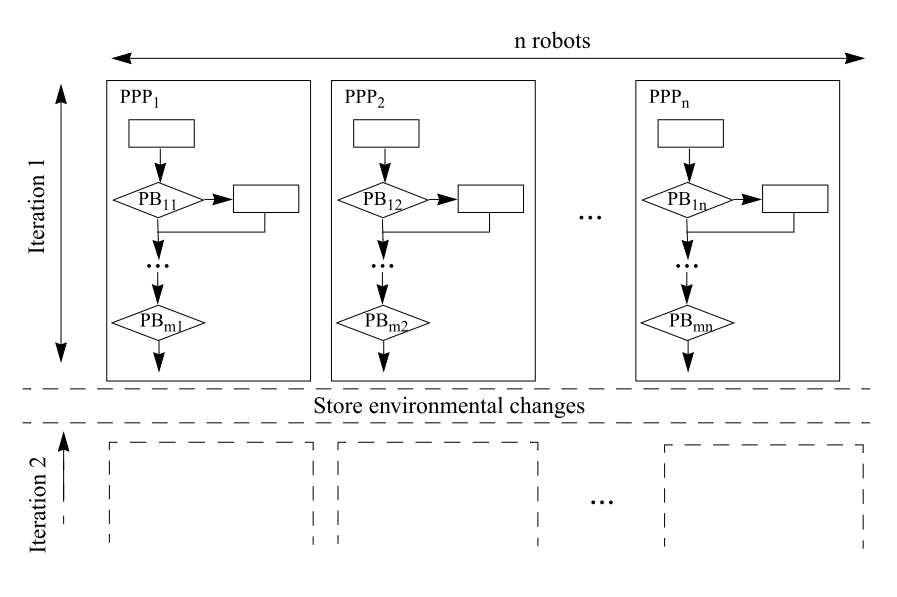
\includegraphics[width=15cm]{martinoliModelMethod.png}
\centering\caption{Gillespie simulation of a swarm system. Each controller, PPP$_i$, describes the independent behavior of a single robot in the swarm. Environmental variables are updated at the end of each iteration.}\label{fig:micromodel}
\end{figure}

We can modify Gillespie's original modeling approach for use with swarm systems---instead of modeling simultaneous molecule interactions we model simultaneous interactions of robot controllers. Martinoli outlines this process in detail in chapter 4.2 of his Ph.D. dissertation\cite{Martinoli1999b} and provides the following concise description,

\begin{quote}
``\emph{[Figure~\ref{fig:micromodel}] shows a general overview of the probabilistic model. The whole simulation consists in running several probabilistic processes in parallel, with one process per robot, while keeping track of the state of the environment. The environment can be seen as a shared memory area (or blackboard) to which all probabilistic processes have access. The state of the robots is defined by a program with exactly the same structure as that of the controllers of the real robots, but, instead of computing the detailed sensory information and trajectories of the robots, the change of states is determined by the throwing of dice (probabilistic blocks). This is an interesting feature of the method because any extension of the real robot controllers can be implemented easily in the probabilistic model and vice versa.}''
\end{quote}

Micro-level simulations are generally not as computationally intensive as solving the rate equations for a macro-model and provide similar results which can, in turn, be used to verify the correctness of the more mathematically and computationally heavy macro-models. This is why micro-level simulations are both, a valuable tool and important step in the design and analysis of swarm systems.

\subsection{Verification of System Properties Using Real Experiments and Physics-Based Simulation}
An important step in any modeling process is verification by comparing model results to real experiment data. Given the relatively abstract approach we have seen so far for designing models of robot swarms, this step is made even more crucial. The micro and macro-models in swarm robotics have conventionally been designed using observed phenomena from other processes seen in biological and chemical systems and adapted to fit the swarming task being studied. Many swarm algorithms show emergent behavior where the observation of complex properties at the system level cannot be trivially inferred from studying the individual agent behavior. The generalizations and simplifications made in the robot controller design when developing the micro and macro-models can, and in many cases do, suppress the interesting emergent properties seen in real physical systems. 

To be able to accurately recreate a task on a swarm system without investing the substantial time and resources required to develop and deploy real robots, we use physics-based simulators. The point of these simulators is to remain as true to the real world as possible while maintaining an order of magnitude improvement in speed and simplicity over real robot experiments. Unlike micro-models that abstract away physical and environmental issues such as wheel slip, sensor noise, communication delays, etc., using probability and dice rolls, physics-based simulators make the added effort to accurately and dynamically model every minute aspect of the swarm system.

\begin{figure}[!ht]
\begin{subfigure}{.5\textwidth}
\centering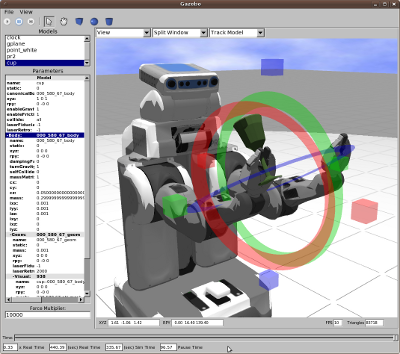
\includegraphics[width=6.5cm]{gazebo.png}
\centering\caption{The Gazebo robot simulator with the PR2 robot.\footnotemark}\label{fig:gazebo}
\end{subfigure}~
\begin{subfigure}{.5\textwidth}
\centering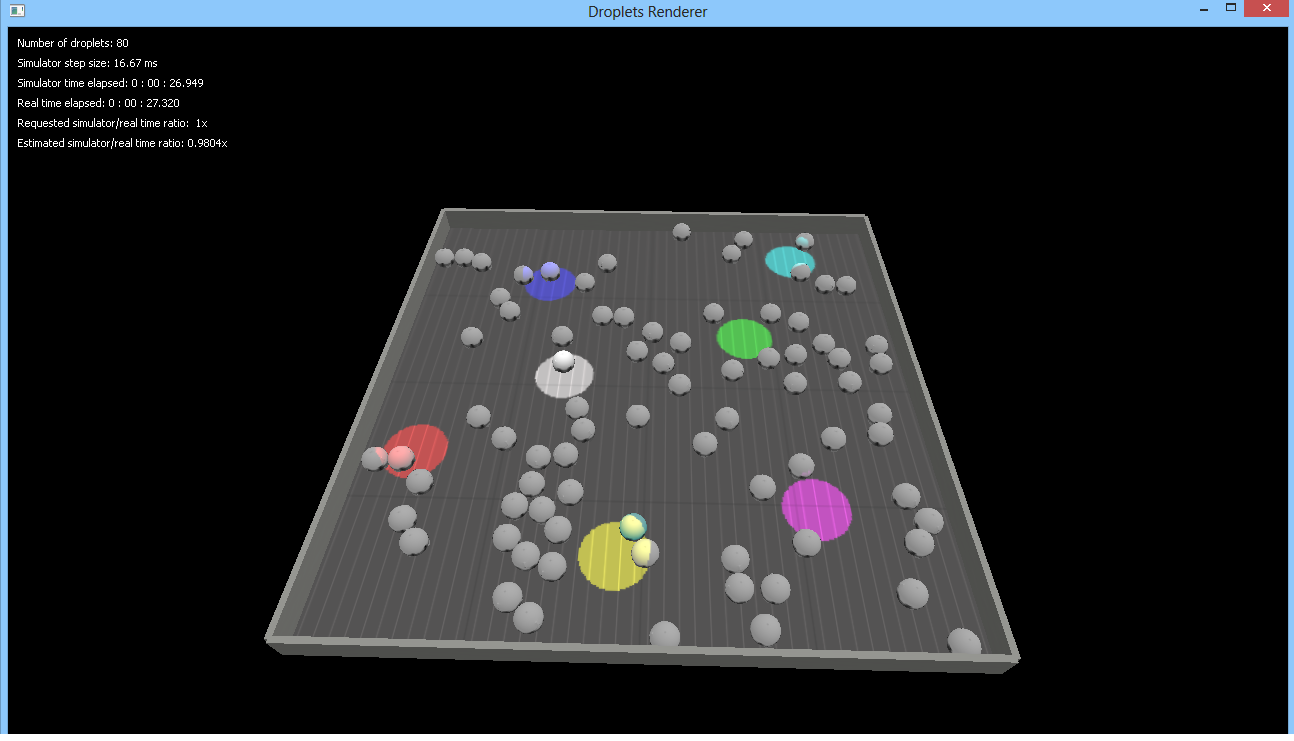
\includegraphics[width=6.5cm]{dsim.png}
\centering\caption{The Droplet swarm robot simulator}\label{fig:dropletsim}
\end{subfigure}
\caption{}
\end{figure}
\footnotetext{Image credit: \texttt{http://ftp.isr.ist.utl.pt/pub/roswiki/simulator\_gazebo.html}}

Many robot simulators are currently available today as either standalone programs like Webots, OpenRAVE and Gazebo (see Figure~\ref{fig:gazebo}) as well as plug-ins and toolkits for popular scientific and engineering software like SolidWorks (Assembly Toolbox), Matlab (Robotics toolbox), Mathematica (SystemModeler) etc. Webots is a widely used simulator in swarm robotics due to its capability to simulate multiple agents and agent-agent/agent-environment interactions in real time. The Webots API also allows for cross-compilation of programs from the simulation environment, right on to real robots without the need for reprogramming and supports a wide range of commercially available robot platforms such as Kilobots, Khepera, Alice, etc. There are also in-house implementations of physics simulators for specific robot platforms, such as the Droplet simulator at Correll Lab seen in Figure~\ref{fig:dropletsim}. 

In almost all swarm robot literature, the results being discussed about a swarming algorithm are backed by simulation data and real experiment data to reinforce the correctness of the algorithm and to verify that it behaves as expected. While this may not sound like a formal verification technique, it is widely used in the robotics community and is generally accepted as a good indication that an algorithm works as described and is often supplied as added conformation along with a more robust mathematical verification of the model.

\subsection{Repeating the Design Loop}
\begin{figure}[!ht]
\centering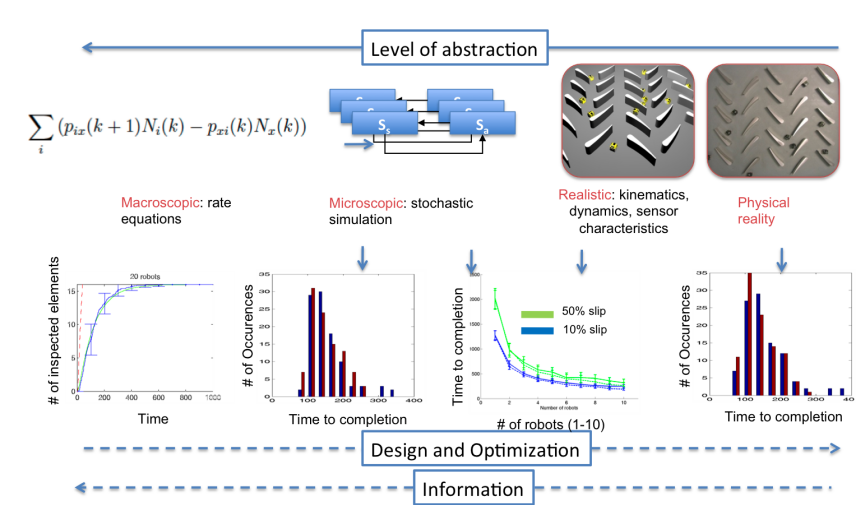
\includegraphics[width=15cm]{modelLoop.png}
\centering\caption{}\label{fig:recipe}
\end{figure}

We have now discussed all the of the steps needed to design a robot controller and its corresponding non-spatial models for a particular swarming task. Figure~\ref{fig:recipe} gives us a visual representation of the entire process including the modeling methods used at different levels of abstraction of the swarm system. 

Lower abstraction levels (right to left in the figure) inform higher abstraction levels by means of calibration and system identification. In turn, higher abstraction levels can be used for designing and optimizing (as we will see in the next section) lower level models and systems. The bottom row of the figure shows selected results (from left to right) for  comparison of rate equation prediction (green) with real robot experiments (blue), the distribution (histogram) for the same data based on stochastic simulation for coordination with (red) and without (blue) communication, the impact of varying amounts of wheel-slip in the Webots simulator (solid lines) and stochastic simulation (dashed lines), and the performance distribution of the real system that closely resembles that obtained from stochastic simulation.

This design methodology is a closed loop feedback system. Setting up the required swarming task as a real physical experiment or physical simulation allows us to discover and measure the different free parameters in the system. We then use these variables in lower resolution models (micro-level) as well as in the development of mathematical models (macro-level) for our system. These, more abstract models allow us to rapidly experiment with system parameters and optimize them. We then use these optimized parameters back in the real physical experiments to improve the desired behavior of the system and repeat the cycle till the desired level of accuracy and satisfaction of  model behavior is achieved. Finally, we hope to deploy these swarm systems in the real world to tackle real problems using the novel yet algorithmically simple approach that swarm robotics lends us.

\subsection{Optimization}\label{sec:opt}
One of the major advantages of the methodology described in this section is the ability to identify and optimize important system parameters. We can re-write the PDM equations in~\eqref{eq:rateeqns} as,
\begin{equation}
S'(\theta,\mu,t) = \Gamma\left(\vec{S}, \theta, \mu, t\right)
\end{equation}
So the temporal evolution of a model is characterized by its state in the past, $\vec{S}(t)$, partially known system parameters ($\theta$), robot control parameters ($\mu$), and time. In other words, the probabilities in eq.\eqref{eq:rateeqns} and eq.\eqref{eq:master} need not be constant values but functions of $\theta$, $\mu$, and $t$.

Two situations commonly arise when designing macro-level models for swarm systems. Firstly, there is the problem of identifying the important system parameters, $\theta$. As pointed out in\cite{Correll2008}, \emph{``In a real robotic system, not all of the model parameters can be known beforehand, either due to uncertainty of measurements or because the chosen model oversimplifies the system (e.g., ignoring friction or sensor noise).''} As such, these parameters are estimated from observations of real experiments and require solving the following optimization problem.
\begin{equation}
	\theta^* = \underset{\overline{\theta}}{\argmin}\left(S^*(\overline{\theta},\mu) - \hat{S}^*(\theta, \mu)\right)^2 \label{eq:thetaopt}
\end{equation}
$S^*(\overline{\theta},\mu)$ is the model prediction of the state vector at steady-state,\\ i.e.~$S^*(\overline{\theta},\mu) = \lim_{t \to \infty}S(\overline{\theta},\mu, t)$, and $\hat{S}^*(\theta, \mu)$ is the experimentally observed state vector at steady-state.

The second situation involves finding optimal control parameters, $\mu$, for a known set of system parameters, $\theta$. The goal is to drive the system towards a desired steady-state distribution, $\tilde{S}^*$, by tuning the model's control parameters. The is accomplished by solving the following optimization problem.
\begin{equation}
	\mu^* = \underset{\overline{\mu}}{\argmin}\left(\tilde{S}^* - S^*(\theta, \overline{\mu})\right)^2 \label{eq:muopt}
\end{equation}

It is evident from eq.\eqref{eq:thetaopt} and eq.\eqref{eq:muopt} that these separate optimization problems are not independent. Starting with initial guesses $\mu(0)$ and $\theta(0)$ alongside simulation results from these guesses, we generate increasingly better values of $\theta$ and $\mu$ for our desired final state distribution $\tilde{S}^*$ using the following recurrence relations.
\begin{align}\label{eq:paramrel}
	\overline{\theta}(n + 1) = & \underset{\overline{\theta}}{\argmin}\sum\limits_{i=0}^{n}\left(S^*(\overline{\theta},\overline{\mu}(i)) - \hat{S}^*(\theta, \overline{\mu}(i), i)\right)^2\\
	\overline{\mu}(n + 1) = & \underset{\overline{\mu}}{\argmin}\left(\tilde{S}^* - S^*(\overline{\theta}(n + 1), \mu)\right)^2
\end{align}
The index $n$ corresponds to the number of the experiment that led to an observation of the steady state $\hat{S}^*(\theta, \mu, n)$. Further discussion and applications of this parameter optimization approach are discussed in\cite{Correll2006a, Correll2008}.
\end{document}